% SPDX-License-Identifier: CC-BY-4.0
%
% Copyright (c) 2023 Nelson Vieira
%
% @author Nelson Vieira <nelson0.vieira@gmail.com>
% @license CC-BY-4.0 <https://creativecommons.org/licenses/by/4.0/legalcode.txt>

\documentclass{scrreprt}
\usepackage{cite}
\usepackage{listings}
\usepackage{underscore}
\usepackage{graphicx}
% \usepackage[tableposition=below]{caption}
% \captionsetup[longtable]{skip=1em}
\usepackage{amsmath,amssymb,amsfonts}
\usepackage{algorithmic}
\usepackage[T1]{fontenc}
\usepackage[table]{xcolor}
\usepackage{adjustbox}
% \usepackage{array,longtable,ltxtable,filecontents}
\usepackage{float}
% \usepackage{showframe}
% \renewcommand*\ShowFrameColor{\color{red}}
\def\UrlBreaks{\do\/\do-}
\def\BibTeX{{\rm B\kern-.05em{\sc i\kern-.025em b}\kern-.08em
    T\kern-.1667em\lower.7ex\hbox{E}\kern-.125emX}}
\usepackage[bookmarks=true]{hyperref}
\usepackage[utf8]{inputenc}
% \usepackage[english]{babel}
\hypersetup{
    bookmarks=false,    % show bookmarks bar?
    pdftitle={Relatório de requisitos de software para Time4People},    % title
    pdfauthor={Nelson Vieira},                     % author
    pdfsubject={Masters Thesis Application},                        % subject of the document
    pdfkeywords={privacy application, internet of things, user empowerment, privacy assistant}, % list of keywords
    colorlinks=true,       % false: boxed links; true: colored links
    linkcolor=blue,       % color of internal links
    citecolor=black,       % color of links to bibliography
    filecolor=black,        % color of file links
    urlcolor=purple,        % color of external links
    linktoc=page            % only page is linked
}%
\def\myversion{alpha 0.3}
\date{}
\usepackage{hyperref}

\begin{document}

\begin{flushright}
    
\includegraphics[width=5cm]{../../thesis/assets/images/uma_logo.png}
    \rule{16cm}{5pt}\vskip1cm
    \Huge{\textbf{\uppercase{Software Requirement}} \\ \textbf{\uppercase{Specification}}} \\
    \vspace{1cm}
    \textbf{for} \\
    \vspace{1cm}
    \textbf{Masters Thesis Application} \\
    \vspace{2cm}
    \LARGE{Version alpha 0.3 \\}
    \vspace{2cm}
    Written by Nelson Vieira \\
    \vspace{2cm}
    \today
    % 22 February 2023
    \vfill
    \rule{16cm}{5pt}
\end{flushright}

\tableofcontents

\chapter{Introduction}

This report aims to define the details and principles of the privacy assisting
IoT application with the ultimate goal of assisting in the development
of the application. Defining the scope of the project helps to understand
the main cases that will be entered. Stakeholders tell us who communicates
with the system directly and indirectly. Business requirements will have
to be defined to know in detail the possibilities of value for both sides.
The swimlane gives a general understanding of the main case and what cause
has each action, the contextual diagram helps to give an understanding
of all actions between the system and the active parties. The data flow
diagram, lets you know in detail what results from the particular activities.
Finally, the technology requirements allow to know how the system will
look like and to define the budget of the work.

\section{The scope and vision of the project}

This project is carried out in the context of the Master's thesis in Informatics
Engineering, which aims to create a mobile application that would provide
information about IoT devices in their surroundings like the type of information
these devices collect and what privacy options are available. The main objective
of this application is to give users another option in order to protect
their private data. The application will show the geolocation of the IoT
devices, what type of device it is, what type of data is being collect by
the device. The application will not detect the devices by itself, this will
be done by the users themselves. As for competition there are other similar
online systems with the same scope as this project. The application offers
an easier search for information about the IoT devices that are around users'
location.

\section{Stakeholders}

A stakeholder can be a person, group, or organisation that is involved in
the project, is affected by its process and outcome or can influence its
process and outcome. Stakeholders can be internal or external to the project
team and the organisation. \cite{fulton2017chapter}
\newline
It is important to identify the stakeholders to make sure you get all the
right requirements for the project and to develop a system that can match
the proposed problem well.
\newline
The following stakeholders are identified in this project:
\begin{itemize}
    \item \textbf{Programmers/designers of the application}: The programmers are the ones who will create the application and even if they do not use it they are directly related to it.
    \item \textbf{IoT Device Owners}: These device owners will be priority stakeholders being that the application in good part will be directed to them, device owners have an indirect influence.
    \item \textbf{Application Users}: The users will be the main focus of this project, they are the ones that provide the information that will be inserted in the application, since they can change the course of the project they have a direct influence.
    \item \textbf{Legislation}: The legislation in relation to the privacy of the collected data allows to impose rules on the use of the data. It has an indirect influence.
\end{itemize}

\chapter{Software requirements}

\section{Business requirements}

Business requirements describe in business terms what must be delivered
or achieved to deliver value. It is what defines the way of doing business,
reflecting the internal policy, the defined process and/or the basic rules
of conduct.  In other words, it is a set of instructions that users already
follow and that the system to be developed must contemplate. Restrictions,
validations, conditions and process exceptions are classic examples of business
rules. A business rule will not necessarily be reflected in the system as
a functionality, but it will certainly determine the behaviour of one or
more functionalities of the system.
\newline
No business requirements have been identified for this project.

\section{Technology requirements}

Technology requirements describe what both hardware and software must be
used in order for a system to be realisable. In terms of hardware, it describes
what kind of physical components are needed for the software to work. The
software to be chosen must take into account the hardware that has been
chosen and what is intended by the stakeholders. This has implications for
how the system is implemented. For example, it is decided that the system
to be implemented should run on iOS smartphones, this implies that the active
stakeholder has to have an iOS smartphone to be able to use the system.
\newline
The technology requirements that have been identified are as follows:
\begin{itemize}
    \item Firestore or similar database server
    \item Programming languages: Dart
    \item Accessible on any smartphone
\end{itemize}
These requirements have been chosen so that the system is available to as
many users as possible regardless of the hardware they use. The database
will allow to store the information that the users provide about the IoT
devices. The application will be developed with Flutter since it uses ahead
of time and just in time compilation with Dart as its programming language.
Flutter has better performance and as such it is the chosen framework for
this application.

\chapter{Contextual diagram}

The contextual diagram aims to establish links between the system under
development and the other actors that interact with the application.
\newline
Identifies the identities external to the application that interact with
the system with data and control between the external entities and the application.
% \begin{figure}[H]
%     \centering
%     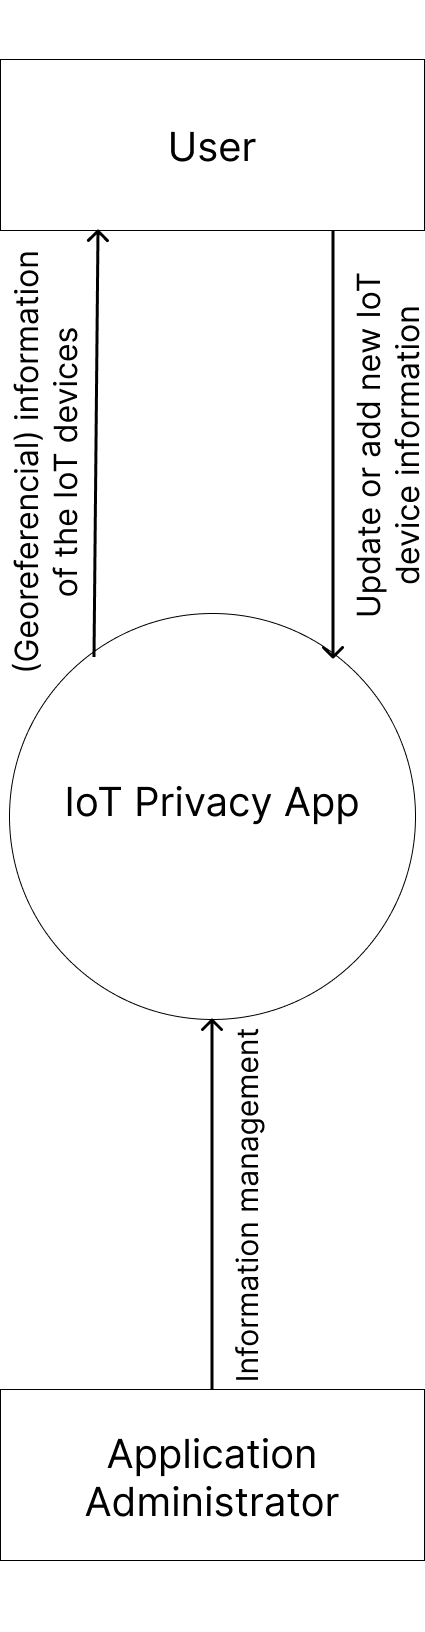
\includegraphics[width=17cm]{assets/contextual_diagram.png}
%     \caption{IoT Privacy Contextual Diagram}
%     \label{fig:contextual diagram}
% \end{figure}
The contextual diagram is based on showing the actions performed with the
application. \\
\newline
User: \\
\newline
→ Receives:

- Profiles/Information of the IoT devices

- Georeference map of the IoT devices
\newline
→ Sends:

- Information update \newline
\newline
Application Administrator: \\
\newline
→ Receive:

- Information from IoT devices
\newline
→ Sends:

- Information management

- Geo-referenced map management

\section{Data flow diagrams}

A data flow diagram shows how information flows between the various entities
in the system and their relationships.
% \begin{figure}[H]
%     \centering
%     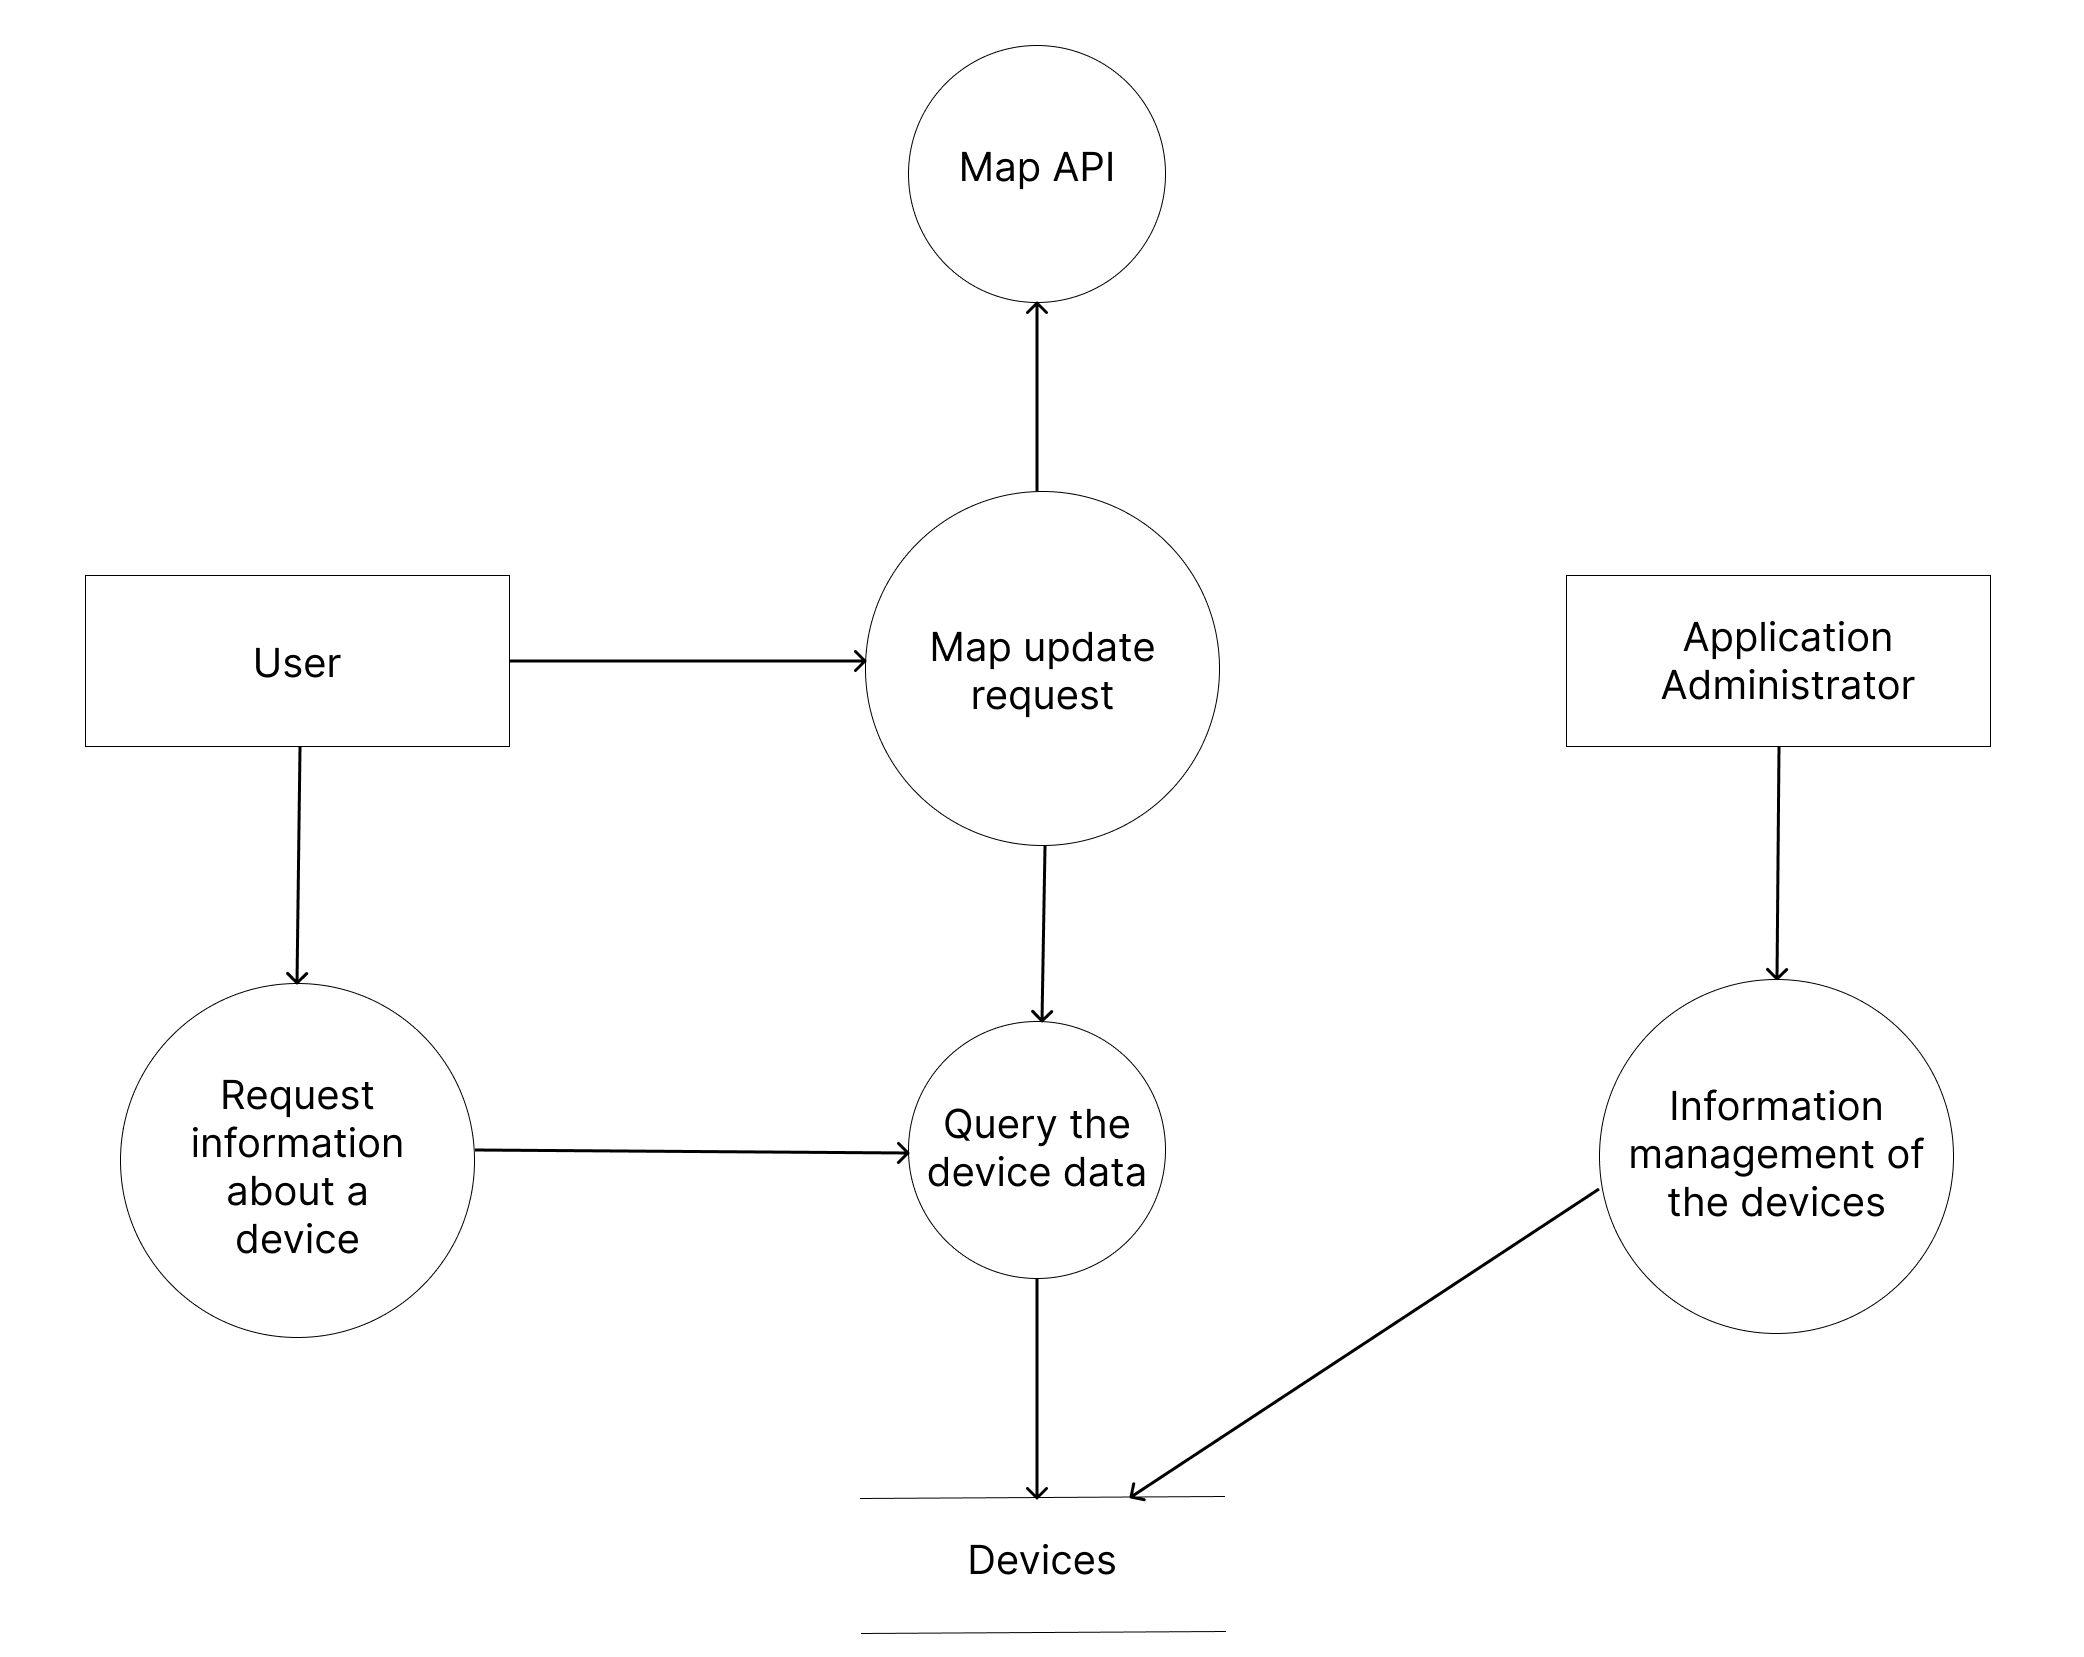
\includegraphics[width=12cm]{assets/data_flow_diagram.png}
%     \caption{Data flow diagram}
%     \label{fig:dataflow_diagram}
% \end{figure}
The user can browse the application map, which will be created with an API,
and see the locations of the IoT devices, the user can also look up information
about the devices by clicking on a device on the map or by searching for
the device in the application. The administrator of the application is responsible for
its maintenance (adding new data, correcting or deleting incorrect data)
and security and for the veracity of the information.

\section{Swimlane diagram (high level)}

A swimlane diagram is a type of flowchart in which processes and decisions
are grouped into lanes. Parallel lines divide the diagram into lanes, each
lane being assigned to people/groups and application.
% \begin{figure}[H]
%     \centering
%     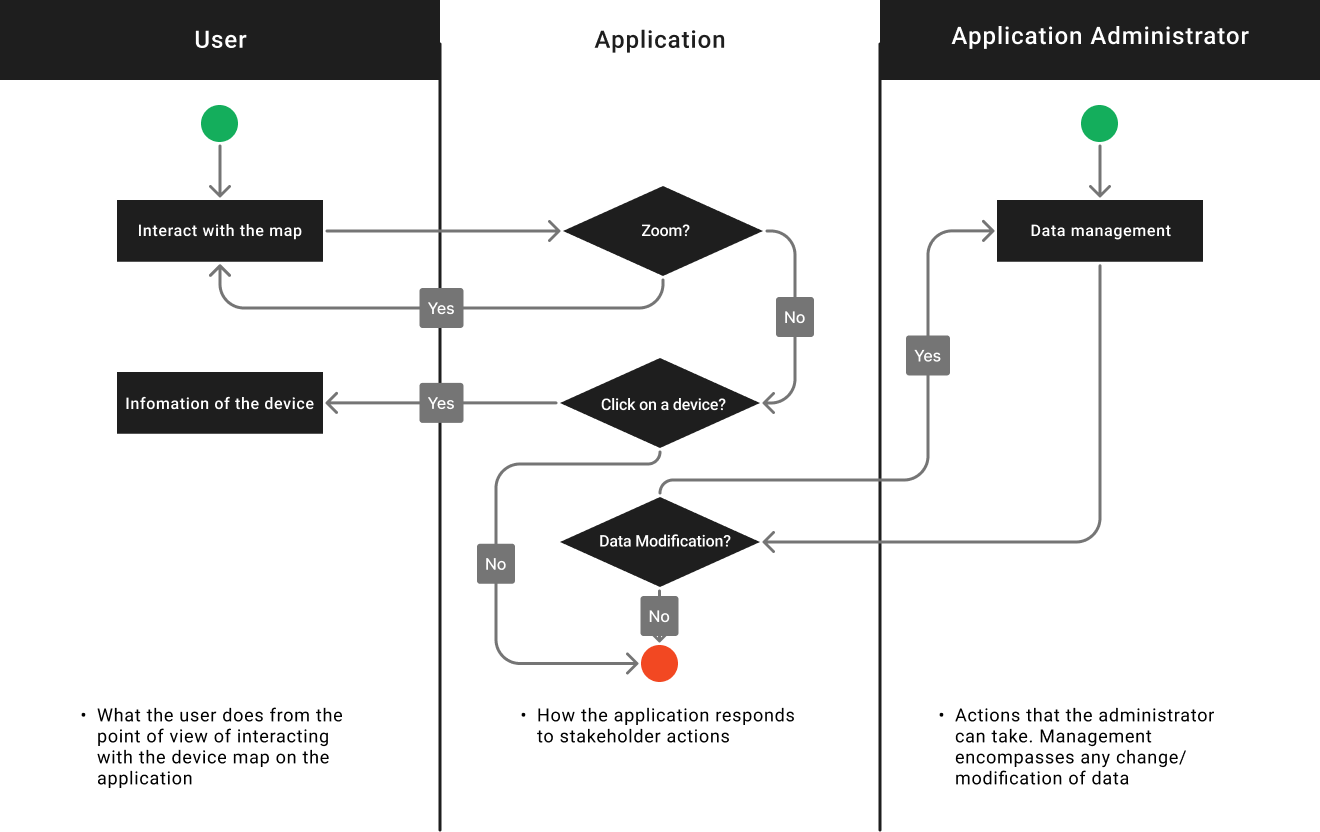
\includegraphics[width=15cm]{assets/swimlane_diagram.png}
%     \caption{Swimlane diagram}
%     \label{fig:diagram_swimlane}
% \end{figure}
This swimlane diagram represents a high level view of a possible user interaction
from the application's map, in this map the user can view the location of
IoT devices and can see more information about a particular device by selecting
it on the map. The application administrator, as mentioned above, can modify the
devices' data.

\section{Requirements table}

The requirements table identifies each feature and links each feature to an origin.
\newline
This is important to make it easier to manage requirements in the future.
Knowing the origin of the creation of the requirements makes it easier to
refer back to the source to clarify any questions.
\newline
A table was created with all the features found. For each feature it was identified
the users to which it is applied and the source.
\newline
For the features found were described the most appropriate requirements for
them. \\
\begin{table}[H]
    \centering
    \begin{adjustbox}{width=1.2\textwidth,center=\textwidth}
    % \rowcolors{5}{gray!10}{gray!40}
    \begin{tabular}{|l|p{0.2\textwidth}|p{0.2\textwidth}|p{0.4\textwidth}|p{0.15\textwidth}|}
        \hline
        \rowcolor{green!20}
        \textbf{R\#} & \textbf{Feature} & \textbf{Applicable stakeholders} & \textbf{Description} & \textbf{Source} \\
        \hline
        \textbf{1} & Navigate the map & User & \textbf{User}: The system should allow the user to scroll through the map of devices & Text \\
        \hline
        \textbf{2} & Select device on the map & User & \textbf{User}: The system should allow the user to select a device on the map to view more information & Text \\
        \hline
        \textbf{3} & Search devices & User & \textbf{User}: The system should allow the user to search for devices by name & Text \\
        \hline
        \textbf{4} & Query devices through parameters & User & \textbf{User}: The system should allow the user to consult devices of only a certain type, data collected, general location & Text \\
        \hline
        \textbf{5} & Query statistics of the devices & User & \textbf{User}: The system should allow consulting statistics of devices & Text \\
        \hline
        \textbf{6} & Add a device & User & \textbf{User}: The system should allow the user to add a new device with name, category, data collected, location, etc. & Text \\
        \hline
        \textbf{7} & Delete a device & App Administrator & \textbf{App Administrator}: The system should allow the administrator to delete a device & Text \\
        \hline
        \textbf{8} & Edit a device & User & \textbf{User}: The system should allow the user to change some data of a device & Text \\
        \hline
        \textbf{9} & Create account & User & \textbf{User}: The system shall allow a user to create an account. & Text \\
        \hline
    \end{tabular}
    \end{adjustbox}
    \caption{Requirements table}
    \label{table:table1}
\end{table}

\section{Functional requirements}

Functional requirements define the functions of a system or its components,
where functions are specifications or behaviours between system outputs and
inputs. \cite{fulton2017chapter} These describe what developers have to implement
so that users can complete tasks (user requirements), which in turn satisfy
business requirements. \cite{wiegers2013software} Functional requirements are
essential to the success of a project.
After building the tracing table the functional requirements that were needed
were extracted for each feature and grouped appropriately according to the
following groups:

\subsection{User Requirements}

\textbf{RU1.1} - The system should allow the user to scroll through the devices map;
\newline
\textbf{RU1.2} - The system shall allow the user to select a device on the map to view more information;
\newline
\textbf{RU1.3} - The system shall allow the user to search for a device by name;
\newline
\textbf{RU1.4} - The system should allow the user to consult devices of only a certain category, data collected, etc.;
\newline
\textbf{RU1.5} - The system must allow consulting statistics of the devices;
\newline
\textbf{RU1.6} - The system should allow the user to add a new device with name, category, data collected, location, etc.;
\newline
\textbf{RU1.7} - The system should allow the user to change some data of a device;
\newline
\textbf{RU1.8} - The system shall allow a user to create an account.

\subsection{Administrator Requirements}

\textbf{RM.2.1} - The system shall allow the administrator to delete an entity;

\subsection{System requirements}

\textbf{RS.4.1} - The system must show statistics related to the devices;

\chapter{Use cases}

\section{Use cases diagram}

The use cases diagram provides a high level visualisation of the user
requirements. The box represents the system boundary. An actor's arrow
for a use case indicates that he is the primary actor for it.
\newline
The primary actor initiates the use case and derives the primary value
from it. An arrow goes from a use case to a secondary actor, where it
participates in some way in the successful completion of the use case. \cite{wiegers2013software}
% \begin{figure}[H]
%     \centering
%     \includegraphics[width=12cm]{assets/diagram_use_cases.png}
%     \caption{Use cases diagram}
%     \label{fig:use cases diagram}
% \end{figure}

\section{Use cases}

In Software Engineering, a use case is a type of classifier representing a
coherent functional unit provided by the system, subsystem, or class manifested
by sequences of interchangeable messages between systems and one or more
actors. \cite{UseUsability}
\newline
Using this technique describes the tasks that users need to perform with
the system or the user-system interaction that may be important to some
stakeholders. They also help in testing by checking that the functionality
has been implemented correctly. The use case uses UML (Unified Modeling
Language) notation.

\begin{table}[H]
    \centering
    \begin{adjustbox}{width=1.2\textwidth,center=\textwidth}
        \begin{tabular}{|m{4cm}|m{12cm}|}
            \hline
            ID and Name: & UC-01 Device information query \\
            \hline
            Created By: & Nelson Vieira 20/02/2023 \\
            \hline
            Primary Actor: & User \\
            \hline
            Description: & The user makes a device information query \\
            \hline
            Trigger: & The user wants to search device information \\
            \hline
            Pre-conditions: & N/A \\
            \hline
            Post-conditions: & POST-1. The user finds device information \\
            \hline
            Normal Flow: & \textbf{1.0 Query information of a device on the map}
            \begin{enumerate}
                \item The user browses the map
                \item The user clicks on the icon to show some information about the device
                \item The user clicks on the device pop-up
            \end{enumerate} \\
            \hline
            Alternative Flow: & \textbf{1.1 Device information search}
            \begin{enumerate}
                \item User enters device name
                \item The user chooses the device he wants from a list generated from the search performed
            \end{enumerate} \\
            \hline
            Alternative Flow: & \textbf{1.2 Alternative search for information from a device}
            \begin{enumerate}
                \item The user selects one of the parameters:
                \begin{enumerate}
                    \item Category
                    \item Data collected
                \end{enumerate}
                \item The user chooses the device he wants from a list generated from the search carried out
            \end{enumerate} \\
            \hline
            Exceptions: & \textbf{1.0.E1  The API is not working}
            \begin{enumerate}
                \item The system displays an alert message: ``We are having connection problems, please wait for a while''
            \end{enumerate} \\
            \hline
            Priority: & High \\
            \hline
            Business Requirements: & N/A \\
            \hline
            Assumptions: & N/A \\
            \hline
        \end{tabular}
    \end{adjustbox}
    \caption{Use case 1 - entity information query}
    \label{use case 1}
\end{table}

\begin{table}[H]
    \centering
    \begin{adjustbox}{width=1.2\textwidth,center=\textwidth}
        \begin{tabular}{|m{4cm}|m{12cm}|}
            \hline
            ID and Name: & UC-02 Device statistics query \\
            \hline
            Created By: & Nelson Vieira 20/02/2023 \\
            \hline
            Primary Actor: & User \\
            \hline
            Description: & The user queries the statistics of the devices \\
            \hline
            Trigger: & The user wants to find statistics of devices \\
            \hline
            Pre-conditions: & N/A \\
            \hline
            Post-conditions: & POST-1. The user finds statistics of devices \\
            \hline
            Normal Flow: & \textbf{2.0 Device statistics query}
            \begin{enumerate}
                \item User selects statistics tab
                \item The user can only select certain parameters, such as:
                \begin{enumerate}
                    \item Category
                    \item Location
                \end{enumerate}
            \end{enumerate} \\
            \hline
            Alternative Flow: & N/A \\
            \hline
            Exceptions: & N/A \\
            \hline
            Priority: & High \\
            \hline
            Business Requirements: & N/A \\
            \hline
            Assumptions: & N/A \\
            \hline
        \end{tabular}
    \end{adjustbox}
    \caption{Use case 2 - statistics query}
    \label{use case 2}
\end{table}

\begin{table}[H]
    \centering
    \begin{adjustbox}{width=1.15\textwidth,center=\textwidth}
        \begin{tabular}{|m{4cm}|m{12cm}|}
            \hline
            ID and Name: & UC-03 Add a device \\
            \hline
            Created By: & Nelson Vieira 22/02/2023 \\
            \hline
            Primary Actor: & User \\
            \hline
            Description: & Addition of a new IoT device in the application \\
            \hline
            Trigger: & The user wants to add a new IoT device \\
            \hline
            Pre-conditions: & N/A \\
            \hline
            Post-conditions: & POST-1. A new IoT device is added to the application \\
            \hline
            Normal Flow: & \textbf{3.0 Add a device}
            \begin{enumerate}
                \item The user enters the following data of a new IoT device:
                \begin{enumerate}
                    \item Name
                    \item Type of data collected
                    \item Category
                    \item Photos
                \end{enumerate}
                \item The user clicks submit
                \item The user adds the location of the IoT device on the map
            \end{enumerate} \\
            \hline
            Alternative Flow: & N/A \\
            \hline
            Exceptions: & \textbf{3.0.E1  The device is already in the database}
            \begin{enumerate}
                \item The system displays an error message
            \end{enumerate} \\
            \hline
            Priority: & High \\
            \hline
            Business Requirements: & N/A \\
            \hline
            Assumptions: & N/A \\
            \hline
        \end{tabular}
    \end{adjustbox}
    \caption{Use case 3 - add a device}
    \label{use case 3}
\end{table}

\begin{table}[H]
    \centering
    \begin{adjustbox}{width=1.1\textwidth,center=\textwidth}
        \begin{tabular}{|m{4cm}|m{12cm}|}
            \hline
            ID and Name: & UC-04 Edit a device's data \\
            \hline
            Created By: & Nelson Vieira 22/02/2023 \\
            \hline
            Primary Actor: & User \\
            \hline
            Description: & Editing the data of an IoT device in the application \\
            \hline
            Trigger: & The user wants to edit an IoT device's data \\
            \hline
            Pre-conditions: & N/A \\
            \hline
            Post-conditions: & POST-1. The data that has been changed appears in the application \\
            \hline
            Normal Flow: & \textbf{4.0 Edit a device's data}
            \begin{enumerate}
                \item The user can change any of the following device data:
                \begin{enumerate}
                    \item Name
                    \item Type of data collected
                    \item Category
                    \item Photos
                \end{enumerate}
                \item The user clicks on submit
            \end{enumerate} \\
            \hline
            Alternative Flow: & N/A \\
            \hline
            Exceptions: &
            % Exceptions: & \textbf{4.0.E1  Unique data already registered}
            % \begin{enumerate}
            %     \item The system displays an error message
            %     \item The system asks the user to enter different data
            % \end{enumerate}
            \textbf{4.0.E1  The device to be edited has been deleted in the meantime}
            \begin{enumerate}
                \item The system displays an error message
                \item The system prohibits editing
            \end{enumerate} \\
            \hline
            Priority: & High \\
            \hline
            Business Requirements: & N/A \\
            \hline
            Assumptions: & N/A \\
            \hline
        \end{tabular}
    \end{adjustbox}
    \caption{Use case 4 - edit a device's data}
    \label{use case 4}
\end{table}

\begin{table}[H]
    \centering
    \begin{adjustbox}{width=1.2\textwidth,center=\textwidth}
        \begin{tabular}{|m{4cm}|m{12cm}|}
            \hline
            ID and Name: & UC-05 Delete a device \\
            \hline
            Created By: & Nelson Vieira 22/02/2023 \\
            \hline
            Primary Actor: & App Administrator \\
            \hline
            Description: & Deleting a device in the application \\
            \hline
            Trigger: & The administrator wants to delete a device \\
            \hline
            Pre-conditions: & PRE-1. The device to be deleted must be in the application's database \\
            \hline
            Post-conditions: & POST-1. The device is deleted from the application \\
            \hline
            Normal Flow: & \textbf{5.0 Delete a device}
            \begin{enumerate}
                \item The administrator deletes a device, through:
                \begin{enumerate}
                    \item ID of device
                    \item Name of device
                \end{enumerate}
                \item The administrator confirms the deletion
                \item The system deletes the device
            \end{enumerate} \\
            \hline
            Alternative Flow: & N/A \\
            \hline
            Exceptions: & \textbf{5.0.E1  The device to be deleted no longer exists in the database}
            \begin{enumerate}
                \item The system displays an error message
                \item The system prohibits deletion
            \end{enumerate} \\
            \hline
            Priority: & High \\
            \hline
            Business Requirements: & N/A \\
            \hline
            Assumptions: & It is assumed that the administrator has database access \\
            \hline
        \end{tabular}
    \end{adjustbox}
    \caption{Use case 5 - delete a device}
    \label{use case 5}
\end{table}


\section{O âmbito e visão do projeto}

Text

\section{Stakeholders}

\chapter{Requisitos de software}

\chapter{Priorização de requisitos}

Em relação à priorização de requisitos, é usada a técnica Quality Function Deployment proposta por Cohen em 1995, que serve para estimar a prioridade de um grupo de requisitos. Baseado no benefício da inclusão de uma feature/requisito, da penalização da mesma não ser incluída e ainda o custo e riscos associados à implementação. Com o método MoSCoW, a partir dos features iniciais é feita ainda uma redução para facilitar o uso da tabela de Quality Function Deployment.
\newline
Nesta abordagem são usados os valores 0 e 1. No caso de 1 significa que o requisito/feature da coluna é mais prioritário que o da linha e se for 0 o contrário verifica-se.

\begin{table}[H]
    \centering
    % \rowcolors{5}{gray!10}{gray!40}
    \begin{tabular}{|>{\columncolor{blue!30!white}}r|r|r|r|r|r|r|r|r|r|}
        \hline
        \rowcolor{blue!30!white}
        \cellcolor{white}Tabela MoSCoW & 1 & 2 & 3 & 4 & 5 & 6 & 7 & 8 & 9 \\
        \hline
        1 && 0 & 0 & 0 & 0 & 0 & 1 & 1 & 0 \\
        \hline
        2 & 1 && 1 & 1 & 0 & 1 & 1 & 0 & 0 \\
        \hline
        3 & 1 & 0 && 0 & 0 & 1 & 1 & 0 & 0 \\
        \hline
        4 & 1 & 0 & 1 && 0 & 1 & 1 & 0 & 0 \\
        \hline
        5 & 1 & 1 & 1 & 1 && 1 & 1 & 1 & 1 \\
        \hline
        6 & 0 & 0 & 0 & 0 & 0 && 1 & 0 & 0 \\
        \hline
        7 & 0 & 0 & 0 & 0 & 0 & 0 && 0 & 0 \\
        \hline
        8 & 1 & 1 & 1 & 1 & 0 & 1 & 1 && 0 \\
        \hline
        9 & 1 & 1 & 1 & 1 & 0 & 1 & 1 & 1 & \\
        \hline
        \rowcolor{green!10}
        Total & 6 & 3 & 5 & 4 & 0 & 7 & 8 & 2 & 1 \\
        \hline
    \end{tabular}
    \caption{Tabela de priorização usando a técnica MoSCoW}
    \label{table:tabela moscow}
\end{table}

Após esta seleção inicial é criada uma tabela de priorização onde é pedido , numa escala de 1-9, para classificar o benefício e penalização de cada requisito. É também estimado o custo e risco de implementação associado a cada feature.

\begin{table}[H]
    \centering
    \begin{adjustbox}{width=1.2\textwidth,center=\textwidth}
    \begin{tabular}{|>{\columncolor{green!10!white}}r|r|r|r|r|r|r|r|r|r|r|}
        \hline
        \rowcolor{blue!20}
        \multicolumn{2}{|c|}{\textbf{Feature}} & \textbf{Benefício relativo} & \textbf{Penalização relativa} & \textbf{Valor Total} & \textbf{Valor \%} & \textbf{Custo relativo} & \textbf{Custo \%} & \textbf{Risco relativo} & \textbf{Risco \%} & \textbf{Prioridade} \\
        \hline
        Eliminar uma entidade & 7 & 7 & 6 & 20 & 10,10 & 1 & 2,56 & 1 & 2,70 & 1,92 \\
        \hline
        Adicionar uma entidade & 6 & 8 & 8 & 22 & 11,11 & 1 & 2,56 & 1 & 2,70 & 2,11 \\
        \hline
        Navegar no mapa & 1 & 9 & 9 & 27 & 13,64 & 8 & 20,51 & 1 & 2,70 & 0,59 \\
        \hline
        Pesquisar entidades & 3 & 8 & 8 & 26 & 13,13 & 6 & 15,38 & 9 & 24,32 & 0,33 \\
        \hline
        Consultar entidades através de parâmetros & 4 & 9 & 7 & 25 & 12,63 & 4 & 10,26 & 2 & 5,41 & 0,81 \\
        \hline
        Selecionar entidade no mapa & 2 & 7 & 7 & 25 & 12,63 & 5 & 12,82 & 1 & 2,70 & 0,81 \\
        \hline
        Editar uma entidade & 8 & 6 & 6 & 18 & 9,09 & 1 & 2,56 & 9 & 24,32 & 0,34 \\
        \hline
        Consultar estatísticas das entidades & 5 & 7 & 6 & 18 & 9,09 & 5 & 12,82 & 4 & 10,81 & 0,38 \\
        \hline
        Criar conta (associada à entidade) & 9 & 6 & 5 & 17 & 8,59 & 8 & 20,51 & 9 & 24,32 & 0,19 \\
        \hline
        \rowcolor{gray!20}
        \multicolumn{2}{|c|}{\textbf{Total}} & 67 & 62 & \textbf{198} & 100,00 & \textbf{39} & 100,00 & \textbf{37} & 100,00 & \\
        \hline
    \end{tabular}
    \end{adjustbox}
    \caption{Tabela de priorização das features}
    \label{table:tabela de priorizacao}
\end{table}

Utilizando este método obtemos os requisitos ordenados por prioridade:

\begin{table}[H]
    \centering
    % \rowcolors{5}{gray!10}{gray!40}
    \begin{tabular}{|c|c|c|c|}
        \hline
        \rowcolor{blue!20!white}
        \textbf{Rank} & \textbf{Feature} & \textbf{\# Feature} & \textbf{Prioridade} \\
        \hline
        1 & Adicionar uma entidade & 6 & 2,11 \\
        \hline
        2 & Eliminar uma entidade & 7 & 1,92 \\
        \hline
        3 & Consultar entidades através de parâmetros & 4 & 0,81 \\
        \hline
        4 & Selecionar entidade no mapa & 2 & 0,81 \\
        \hline
        5 & Navegar no mapa & 1 & 0,59 \\
        \hline
        6 & Consultar estatísticas das entidades & 5 & 0,38 \\
        \hline
        7 & Editar uma entidade & 8 & 0,34 \\
        \hline
        8 & Pesquisar entidades & 3 & 0,33 \\
        \hline
        9 & Criar conta (associada à entidade) & 9 & 0,19 \\
        \hline
    \end{tabular}
    \caption{Requisitos mais prioritários ordenados}
    \label{table:requisitos ordenados}
\end{table}

\section{Critérios de aceitação}

Para mais facilmente conseguir-se testar se as features mais prioritárias que foram escolhidas anteriormente foram bem implementadas foram criados estes critérios de aceitação para cada uma delas. Estes critérios ajudam-nos a perceber as condições mínimas para que esta aplicação possa ser considerada um MVP, “minimum viable product”, ou seja, para que este projeto tenha os requisitos mínimos possíveis de forma a que este seja considerado production ready.
\newline
Para estes critérios de aceitação foi considerado o seguinte:

\begin{itemize}
    \item Funcionalidade de alto nível que tem de estar presente para que o sistema seja usável
    \item Critérios não funcionais e métricas de qualidade que têm de ser satisfeitas
    \item Possibilidade de problemas em aberto ou defeitos (podemos garantir que nenhum defeito ou TBD esteja presente para o sistema ser aceite)
    \item Restrições legais ou contratuais (que têm de ser satisfeitas para o sistema ser aceite)
\end{itemize}

\subsection{Features}

\subsubsection{Eliminar uma entidade}

\begin{itemize}
    \item O sistema deverá permitir a eliminação de uma entidade
\end{itemize}

\subsubsection{Adicionar uma entidade}

\begin{itemize}
    \item O sistema permite ao Gestor do Portal adicionar uma entidade com os seguintes parâmetros: nome, NIF, morada, contactos (site, email, telefone, redes sociais), natureza jurídica, estatuto jurídico, data de criação, âmbito geográfico, área de intervenção
\end{itemize}

\subsubsection{Navegar no mapa}

\begin{itemize}
    \item O sistema consegue representar as entidades da região no mapa
\end{itemize}

\subsubsection{Pesquisar entidades}

\begin{itemize}
    \item O sistema permite pesquisar entidades pelo nome
\end{itemize}

\subsubsection{Consultar entidades através de parâmetros}

\begin{itemize}
    \item O sistema permite pesquisar entidades pelos seguintes parâmetros: NIF, morada, natureza jurídica, estatuto jurídico, data de criação, âmbito geográfico, área de intervenção
\end{itemize}

\subsubsection{Selecionar entidade no mapa}

\begin{itemize}
    \item O sistema permite a selecionar uma entidade no mapa
\end{itemize}

\subsubsection{Editar uma entidade}

\begin{itemize}
    \item O sistema permite a edição de uma entidade
    \item O sistema guarda na base de dados as modificações que foram realizadas
\end{itemize}

\subsubsection{Consultar estatísticas das entidades}

\begin{itemize}
    \item O sistema permite que o utilizador possa consultar estatísticas relativas às entidades
\end{itemize}

\subsubsection{Criar conta (associada à entidade)}

\begin{itemize}
    \item O sistema consegue criar um novo perfil do tipo Entidade
    \item A Entidade tem que inserir o seu nome, NIF, morada, nº de telefone, email e uma password
    \item O sistema consegue detectar se o email já está em uso
    \item O sistema consegue detectar se o NIF da entidade já está em uso
    \item O sistema consegue enviar email de confirmação de criação de perfil
    \item O utilizador consegue confirmar criação de perfil
\end{itemize}

\section{Protótipo}

Para o protótipo é realizado primeiramente vários drafts com
ferramentas de design, como Figma ou . Depois, com as ferramentas
referidas anteriormente em \textbf{Requisitos de Tecnologia} (PHP,
HTML, CSS e Javascript), é criado um website.

\bibliographystyle{IEEEtran}
\bibliography{assets/references}

\end{document}
